\section{Partición en clusters}

\par Implementamos diferentes algoritmos para la detección de comunidades en la red de delfines. La asignación de cada algoritmo se puede observar en la figura \ref{fig:Layouts_clusters}, en la cual se puede observar que todos los algoritmos detectan entre 4 y 6 comunidades presentes en la red, aunque en algunos casos aparecen comunidades compuestas por solo dos delfines, es decir, de un tamaño considerablemente menor que el las restantes, lo cual se podría considerar la absorción de esta pequeña comunidad por parte de otra de mayor tamaño.
\par En la tabla \red{table:Modularidad} calculamos la modularidad y el silhouette dada por cada algoritmo, 

\begin{figure}
\centering
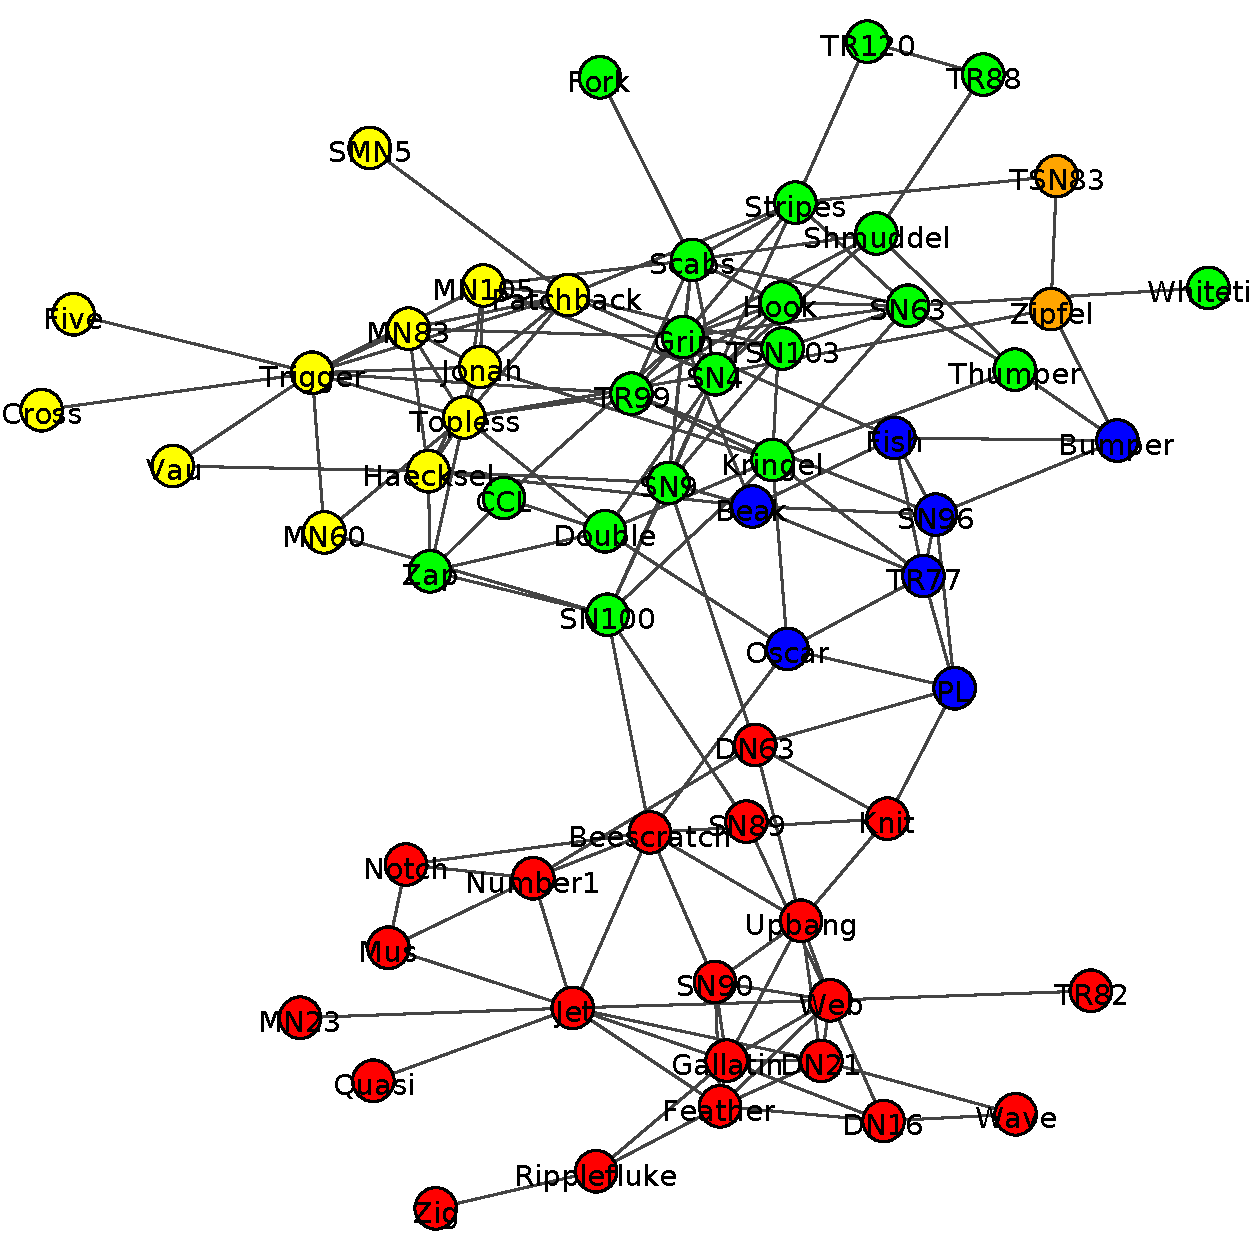
\includegraphics[scale = 0.2]{figuras/Edge_betweenness}
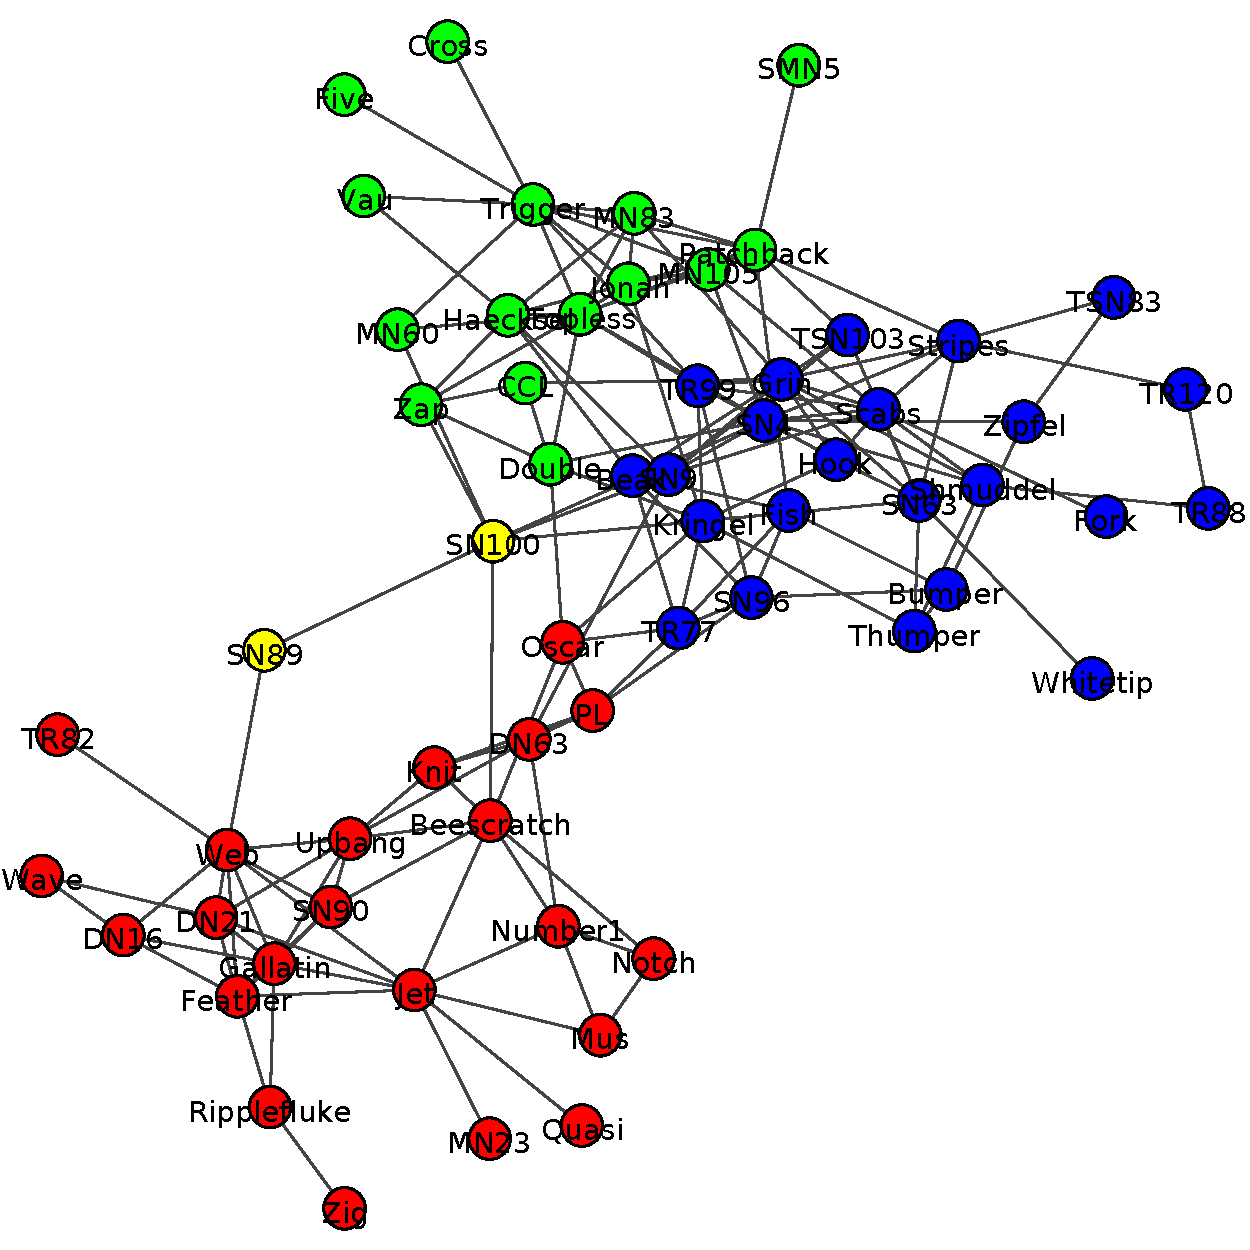
\includegraphics[scale = 0.2]{figuras/Fast_greedy} \\
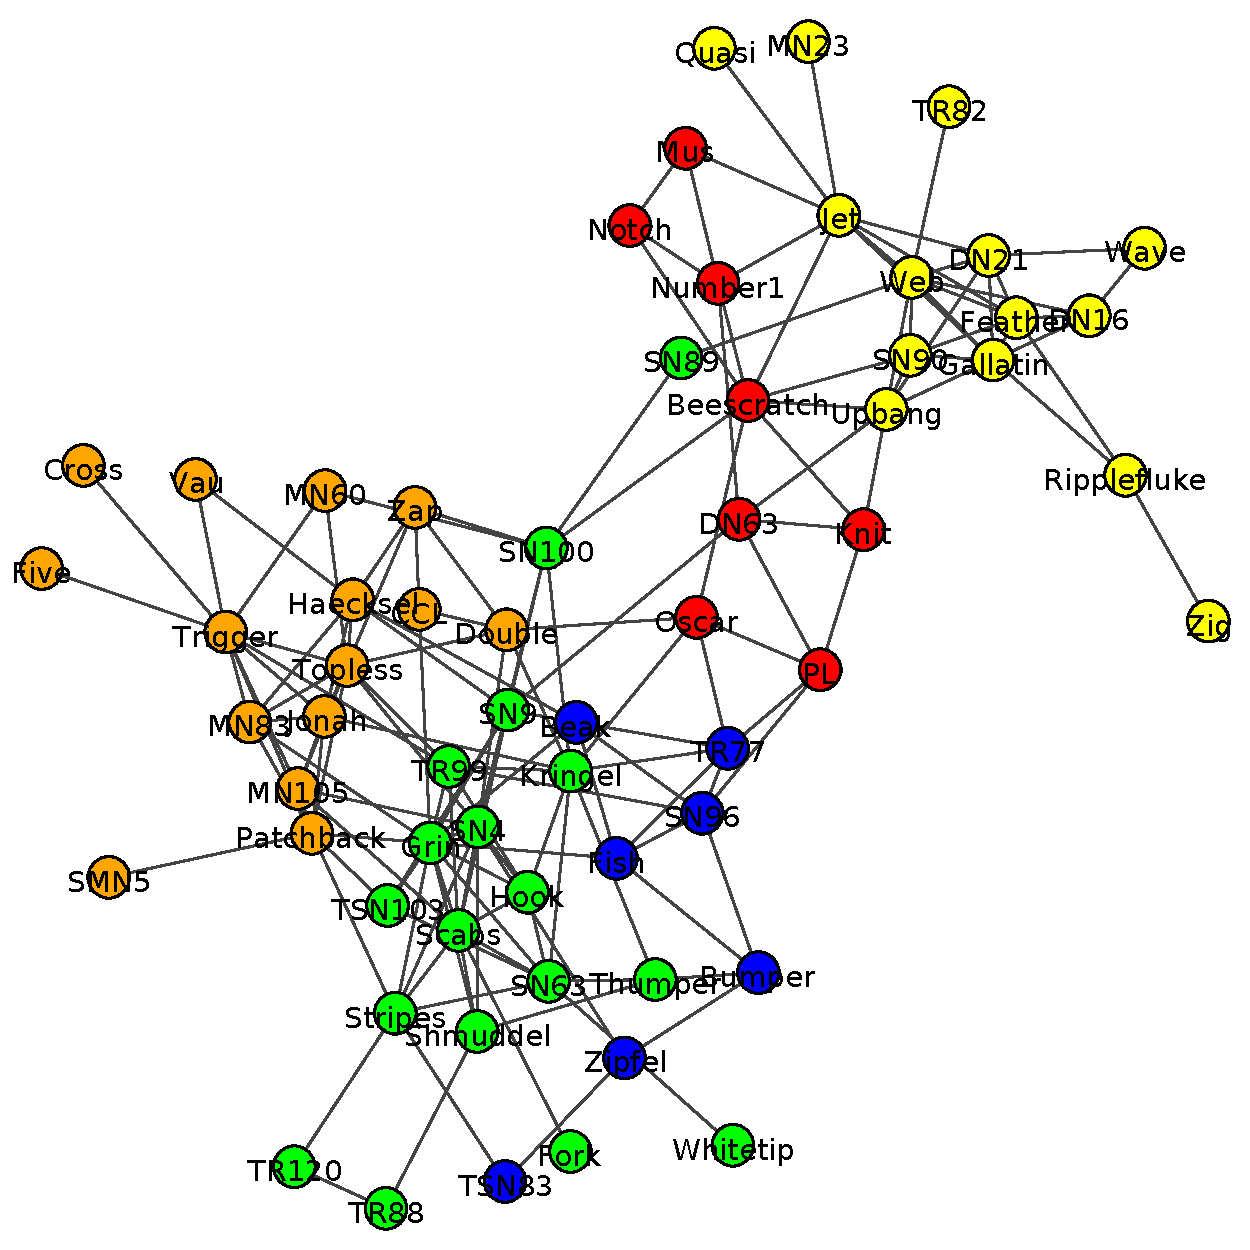
\includegraphics[scale = 0.2]{figuras/Louvain}
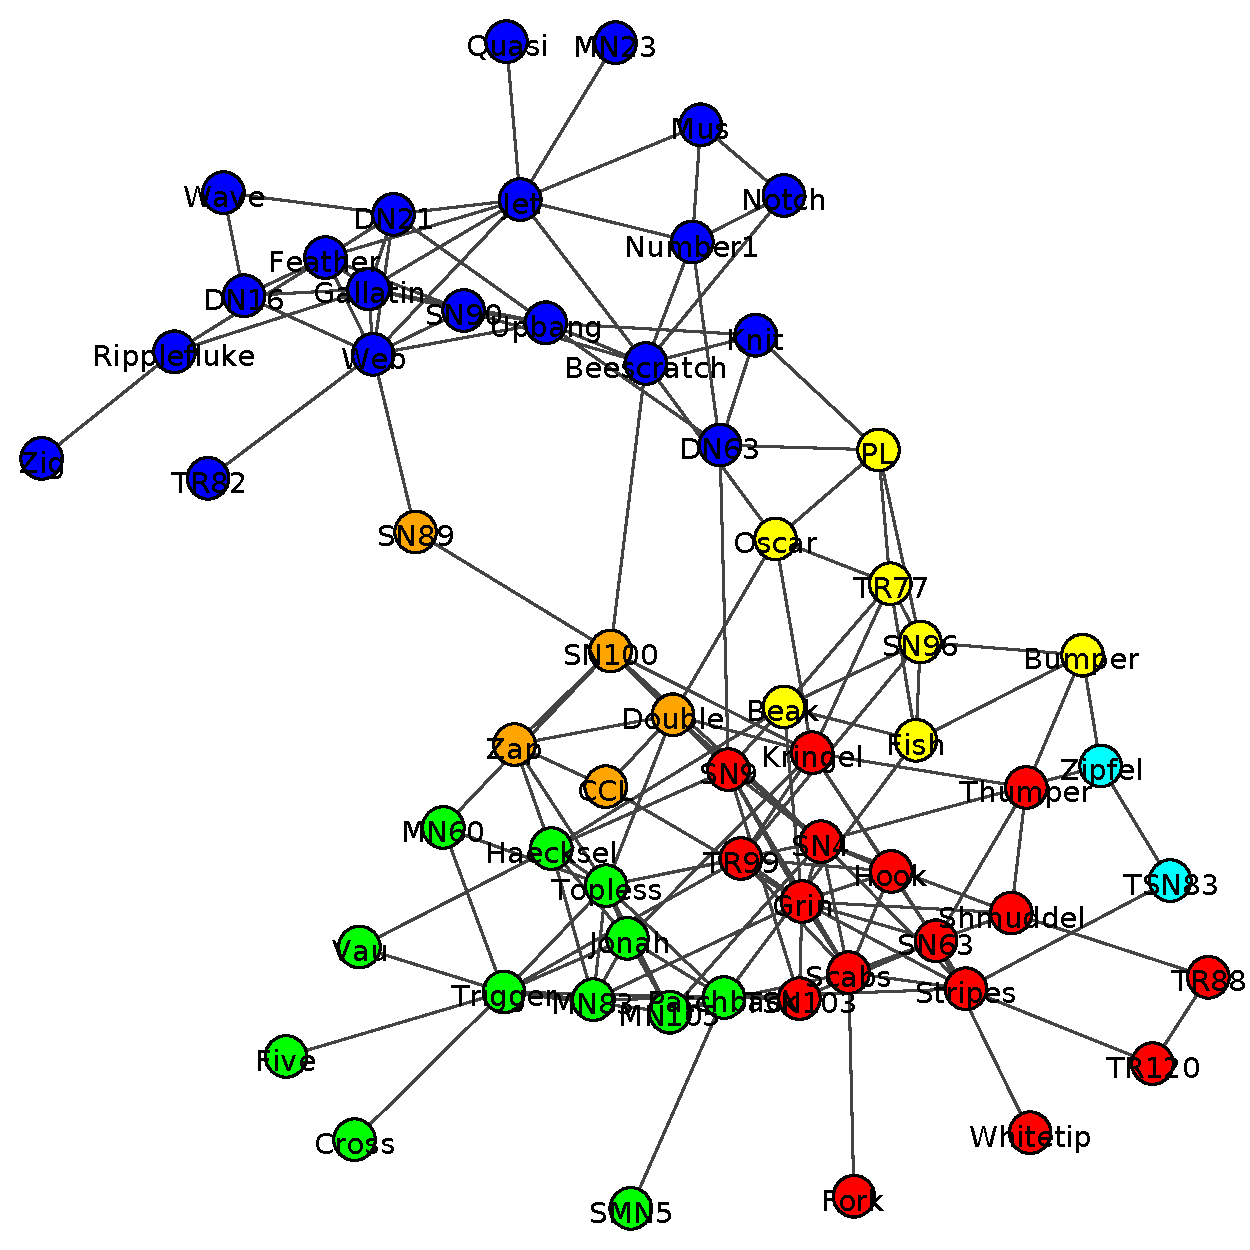
\includegraphics[scale = 0.2]{figuras/Infomap}
\caption{Layouts indicando el cluster asignado por cada algoritmo.}
\label{fig:Layouts_clusters}
\end{figure}

\section{Modularidad}

\begin{table}
\centering
\begin{tabular}{c c c}
\hline \hline
Algoritmo & Modularidad & Silhouette \\
\hline
Edge-betweenness & 0.519 & 0.338 \\
Fast greddy & 0.495 & 0.184 \\
Louvain & 0.519 & 0.294 \\
Infomap & 0.529 & 0.328 \\
\hline\hline
\end{tabular}
\caption{Modularidad y Silhouette de las particiones dadas por diferentes algoritmos.}
\label{table:Modularidad}
\end{table}


\begin{figure}
\centering
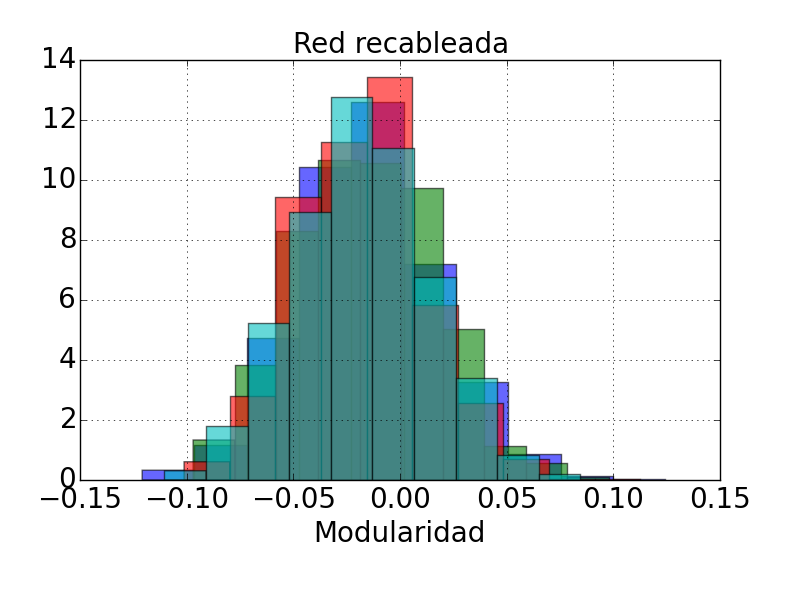
\includegraphics[scale = 0.5]{figuras/Modularidad_random}
\includegraphics[scale = 0.5]{figuras/Silhouette_random}
\caption{Modularidad y Silhouette recableando en forma aleatoria, manteniendo la pertenencia a cada cluster dada por los algoritmos de detección de particiones.Se puede observar que la probabilidad de obtener los valores de la tabla \ref{table:Modularidad} dada una reconexión aleatoria es prácticamente nula.}
\label{fig:Modularidad_random}
\end{figure}
